\documentclass[12pt,a4paper]{article}

%% Packages
\usepackage{amsmath,amssymb,amsthm}
\usepackage{mathtools}
\usepackage[T1]{fontenc}
\usepackage{geometry}
\geometry{margin=1.2in}
\usepackage{microtype}
\usepackage{hyperref}
\hypersetup{colorlinks=true, linkcolor=black, citecolor=black, urlcolor=black}
\usepackage{cleveref}
\usepackage{booktabs}
\usepackage{graphicx}
\usepackage{enumitem}
\usepackage{setspace}
\onehalfspacing
\usepackage{titlesec}
\usepackage{abstract}

%% Theorem environments
\newtheorem{theorem}{Theorem}[section]
\newtheorem{corollary}[theorem]{Corollary}
\newtheorem{proposition}[theorem]{Proposition}
\newtheorem{definition}[theorem]{Definition}
\theoremstyle{remark}
\newtheorem{remark}[theorem]{Remark}

%% Shorthand

\newcommand{\vv}{\mathbf{v}}
\newcommand{\Rcal}{\mathcal{R}}
\newcommand{\Acal}{\mathcal{A}}
\newcommand{\Bcal}{\mathcal{B}}
\newcommand{\Lcal}{\mathcal{L}}
\newcommand{\reff}{r_{\mathrm{eff}}}
\newcommand{\dL}{d_L^{\mathrm{RSVP}}}
\newcommand{\DAr}{D_A^{\mathrm{RSVP}}}
\newcommand{\DHr}{D_H^{\mathrm{RSVP}}}
\newcommand{\DMr}{D_M^{\mathrm{RSVP}}}
\newcommand{\DVr}{D_V^{\mathrm{RSVP}}}
\newcommand{\Heff}{H_{\mathrm{eff}}}
\newcommand{\rhoRSVP}{\rho_{\mathrm{RSVP}}}
\newcommand{\pRSVP}{p_{\mathrm{RSVP}}}
\newcommand{\weff}{w_{\mathrm{eff}}}
\newcommand{\ceff}{c_{\mathrm{eff}}}

\title{\textbf{Cosmological Observables Without Expansion:\\
A Scalar--Vector--Entropy Field Theory of Redshift,\\
Luminosity Distance, and the Hubble Tension}\\[1em]
{\large An RSVP and Spherepop Synthesis}}

\author{Flyxion\\
\small Chief Curriculum Architect of Computational Philosophy}

\date{2026}

\begin{document}

\maketitle

\begin{abstract}
We develop a formal cosmological framework, the Relativistic Scalar--Vector--Plenum (RSVP) theory, in which the standard observables of modern cosmology---redshift, luminosity distance, baryon acoustic oscillations, angular diameter distance, and gravitational lensing---arise from propagation through a structured scalar--vector--entropy field rather than from the expansion of a metric. The framework replaces the Friedmann scale factor as the primary dynamical variable with three coupled fields: a scalar constraint-density field $\Phi$, a vector transport field $\vv$, and an entropy field $S$. The standard hierarchy of dark-energy cosmologies---$\Lambda$CDM, $w$CDM, $w_0 w_a$CDM, $\phi$CDM, and interacting dark-energy models---is shown to constitute a nested sequence of truncations of the full RSVP dynamics. We define a relaxation functional $\Rcal$, derived from the RSVP field equations, that generates both redshift and effective distance without presupposing an expanding geometry. A degeneracy theorem establishes that RSVP is observationally indistinguishable from Friedmann cosmology when $\Rcal$ is homogeneous and slowly varying, while a companion corollary identifies five distinct observational signatures that break the degeneracy when $\Rcal$ varies across lines of sight or environments. We then ground the entire framework in the Spherepop irreversible event calculus, showing that cosmological redshift is a direct measure of accumulated irreversible interaction history along photon trajectories, and that the cosmological arrow of time emerges from the monotonic growth of event histories rather than from global boundary conditions. The persistent Hubble tension is interpreted as a projection mismatch arising from different observational probes sampling different field regimes. The framework provides a coherent alternative ontology for cosmological observation while remaining testable through probe-dependent $H_0$ anisotropy, environment-dependent BAO distortions, and lensing signals correlated with entropy gradients beyond matter density alone.
\end{abstract}

\tableofcontents
\newpage

%%=============================================================
\section{Introduction}
%%=============================================================

The discovery of accelerating cosmic expansion at the close of the twentieth century established the cosmological constant $\Lambda$ as the dominant component of the energy budget of the late universe. Subsequent decades of observation have refined but not resolved the foundational questions this discovery raised: what is the physical nature of dark energy, why does it take the value it does, and why does its energy density coincide with that of matter at the present epoch? These questions have motivated an extensive program of model comparison, using increasingly precise data from cosmic microwave background (CMB) anisotropies, baryon acoustic oscillations (BAO), and Type~Ia supernovae.

A recent comprehensive analysis by Zhang, Xu, and Chen~\cite{zhang2026} using DESI DR2 BAO, Pantheon+, and Planck~2018 plus ACT DR6 CMB and lensing data has sharpened the empirical situation considerably. That study compares five cosmological models---$\Lambda$CDM, $w$CDM, $w_0 w_a$CDM, $\phi$CDM, and a $\xi$-index interacting dark-energy model---and finds three key results. First, the Hubble constant inferred from combined data consistently aligns with early-universe measurements across all models, indicating that the Hubble tension persists regardless of dark-energy parameterization. Second, there is compelling evidence for dynamical dark energy: early-universe CMB data prefer a phantom equation-of-state parameter $w < -1$, while late-universe BAO and supernova data prefer quintessence $w > -1$. Third, the full data set suggests a late-time energy transfer between dark energy and matter. None of the tested models, however, resolves the Hubble tension, and none achieves decisive Bayesian preference over $\Lambda$CDM across all data combinations.

The present paper argues that this pattern of success-yet-failure is not a contingent failure of the models tested, but a structural consequence of their shared ontological commitment: all five models assume that the universe is described by a homogeneous expanding metric, with dark energy modeled as a fluid or scalar field evolving within that geometry. Observations are then interpreted as measuring the kinematics of that expansion. If this assumption is wrong---not falsified, but insufficiently general---then improving the fluid parameterization will never resolve the underlying tensions.

We propose an alternative framework, the Relativistic Scalar--Vector--Plenum (RSVP) theory, in which cosmic evolution is described by three coupled fields on a large-scale manifold: a scalar constraint-density field $\Phi$, a vector transport field $\vv$, and an entropy field $S$. What standard cosmology interprets as expansion is, in RSVP, the coarse-grained kinematic projection of a structured plenum undergoing constraint relaxation, transport, and entropy redistribution. The observed Hubble law is an emergent approximation, not a fundamental fact of geometry.

We also draw on two related proposals that point in the same direction. The entropic expansion principle of Joustra~\cite{joustra} correctly identifies entropy growth, particularly black hole entropy, as a constitutive driver of large-scale cosmic behavior, and attempts to tie cosmic expansion directly to entropy increase. This proposal captures something genuine but remains underdetermined: a scalar entropy driver cannot explain the phantom-to-quintessence transition, the effective dark-sector coupling, or the epoch-dependent Hubble inference observed in the data. RSVP generalizes this insight by embedding entropy within a richer three-field dynamical system.

Finally, we ground the entire framework in the Spherepop irreversible event calculus~\cite{spherepop}, which defines systems not in terms of reversible states but in terms of append-only event histories. This provides a formal substrate for understanding why propagation through an RSVP field induces redshift: not as wavelength stretching by expanding space, but as the accumulation of irreversible interaction events along photon trajectories.

The paper is organized as follows. Section~\ref{sec:fields} introduces the RSVP field equations. Section~\ref{sec:truncation} shows how standard dark-energy models arise as truncations of RSVP. Section~\ref{sec:relaxation} defines and constrains the relaxation functional. Section~\ref{sec:degeneracy} states and proves the degeneracy theorem and its corollary. Section~\ref{sec:redshift} derives the RSVP redshift law. Section~\ref{sec:luminosity} derives the luminosity distance. Section~\ref{sec:bao} treats BAO and angular diameter distance. Section~\ref{sec:lensing} addresses gravitational lensing. Section~\ref{sec:spherepop} establishes the Spherepop foundation for irreversibility and the arrow of time. Section~\ref{sec:hubble} interprets the Hubble tension. Section~\ref{sec:conclusion} summarizes and identifies future directions.

%%=============================================================
\section{RSVP Field Equations}
\label{sec:fields}
%%=============================================================

\subsection{Motivation and Field Content}

Standard cosmology treats the scale factor $a(t)$ as the primary dynamical variable and encodes the large-scale evolution of the universe through the Friedmann equations. This procedure has proven empirically powerful, but it remains ontologically thin. It presupposes that the large-scale universe is best described by homogeneous fluids whose behavior can be summarized by a few scalar parameters, even when observational data increasingly suggest redshift-dependent evolution, possible dark-sector coupling, and persistent inconsistencies between early- and late-universe inferences.

The RSVP framework begins from a different premise. It models cosmic evolution as the coarse-grained outcome of a deeper scalar--vector--entropy dynamics. In this view, what standard cosmology interprets as expansion is an effective projection of a structured plenum undergoing constraint relaxation, transport, and entropy redistribution.

Let the cosmological substrate be described by three coupled fields on a large-scale manifold $\mathcal{M}$:
\begin{equation}
\Phi(x,t) \in \mathbb{R}, \qquad \vv(x,t) \in T\mathcal{M}, \qquad S(x,t) \in \mathbb{R}.
\end{equation}
These fields are not three independent substances. They are three coupled aspects of a single evolving substrate:
\begin{enumerate}[leftmargin=2em]
\item $\Phi$ is the \emph{scalar constraint-density field}: local plenum compression, structural loading, or stored configurational tension.
\item $\vv$ is the \emph{vector transport field}: directed relaxation, organized redistribution, or coherent flow.
\item $S$ is the \emph{entropy field}: local disorder production, smoothing pressure, or dissipation of structured gradients.
\end{enumerate}
Matter and radiation appear not as independent cosmological fluids at the fundamental level, but as coarse-grained excitations or emergent observables derived from particular regimes of $(\Phi, \vv, S)$.

\subsection{Fundamental Evolution Equations}

The large-scale RSVP dynamics are governed by the coupled system:
\begin{align}
\partial_t \Phi + \nabla \cdot (\Phi \vv) &= D_\Phi \nabla^2 \Phi
  - \alpha_\Phi \frac{\delta \mathcal{U}}{\delta \Phi}
  - \beta_\Phi \,\Xi(\Phi,S), \label{eq:phi} \\[0.5em]
\partial_t \vv + (\vv\cdot\nabla)\vv &= -\nabla \Psi(\Phi,S) - \gamma \vv
  + \nu \nabla^2 \vv + \mathbf{T}(\Phi,\vv,S), \label{eq:v} \\[0.5em]
\partial_t S + \nabla\cdot(S\vv) &= D_S \nabla^2 S + \sigma(\Phi,\vv,S),
  \qquad \sigma \ge 0. \label{eq:S}
\end{align}
The terms have the following interpretations. In \eqref{eq:phi}, $D_\Phi \nabla^2 \Phi$ describes scalar smoothing, $\mathcal{U}(\Phi)$ is a structural potential governing local constraint landscapes, and $\Xi(\Phi,S)$ represents scalar-to-entropy conversion or relaxation. In \eqref{eq:v}, the effective drive $-\nabla\Psi(\Phi,S)$ determines how scalar and entropic gradients induce directed transport; $\gamma$ is a damping coefficient; $\nu$ is a viscosity-like term; and $\mathbf{T}$ captures higher-order torsion, vorticity, or coherence-preserving transport. In \eqref{eq:S}, $D_S \nabla^2 S$ describes entropy diffusion and $\sigma$ is the local entropy-production functional. The condition $\sigma \ge 0$ enforces a generalized second-law structure at the field level.

\subsection{Emergent Cosmological Kinematics}

In RSVP, one does not begin with a scale factor. Instead, one derives an effective scale description by coarse-graining the field dynamics over sufficiently large domains $\mathcal{D}$. Let angle brackets denote spatial averaging over such a domain. Define the effective cosmological expansion rate by
\begin{equation}
\Theta_{\mathrm{eff}}(t) = \langle \nabla \cdot \vv \rangle, \qquad
\Heff(t) = \frac{1}{3}\,\Theta_{\mathrm{eff}}(t).
\end{equation}
If one wishes, an effective scale factor $a_{\mathrm{eff}}(t)$ may then be introduced secondarily by
\begin{equation}
\frac{\dot a_{\mathrm{eff}}}{a_{\mathrm{eff}}} = \Heff(t).
\end{equation}
This is the decisive ontological reversal. In Friedmann cosmology, geometry drives matter evolution. In RSVP, structured field evolution induces an effective large-scale geometry. The metric-like behavior inferred observationally is a projection of deeper field organization.

\subsection{Field Closure: Potentials and Structural Constraints}

For the RSVP field equations to constitute a closed theory rather than a
framework, the structural potential $\mathcal{U}(\Phi)$ and the effective drive
$\Psi(\Phi, S)$ must be specified or constrained. We adopt the minimal closures
consistent with two requirements: recovery of $\Lambda$CDM in the frozen limit,
and a well-posed stability structure for the scalar sector.

\paragraph{Structural potential.}
We adopt a double-well ansatz
\begin{equation}
\mathcal{U}(\Phi) = \frac{\lambda_\Phi}{4}(\Phi^2 - \Phi_0^2)^2,
\label{eq:U}
\end{equation}
where $\Phi_0$ is the equilibrium constraint density and $\lambda_\Phi > 0$
is a stiffness coefficient. This potential has two stable minima at
$\Phi = \pm\Phi_0$ separated by an unstable ridge at $\Phi = 0$, which encodes
the physical idea that the plenum has a preferred structural loading. The
$\Lambda$CDM limit corresponds to $\Phi \approx \Phi_0$ (frozen near a minimum),
in which case $\delta\mathcal{U}/\delta\Phi \approx 0$ and the scalar equation
reduces to a pure diffusion--advection law.

\paragraph{Effective drive.}
The drive potential coupling scalar and entropy fields is taken to be
\begin{equation}
\Psi(\Phi, S) = \frac{\partial \mathcal{U}}{\partial \Phi} + \lambda_S S
= \lambda_\Phi \Phi(\Phi^2 - \Phi_0^2) + \lambda_S S,
\label{eq:Psi}
\end{equation}
where $\lambda_S > 0$ couples entropy gradients to transport flow. This
ensures that regions of elevated entropy production drive directed relaxation
flows, realizing the physical picture of entropy-mediated redistribution in
the plenum.

\paragraph{Recovery of Friedmann in the truncated limit.}
Under the substitutions $\partial_t\Phi \approx 0$, $\vv \approx 0$,
$\partial_t S \approx 0$, and the identification
\begin{equation}
\rhoRSVP \to \rho_{\mathrm{tot}},
\qquad
\pRSVP \to p_{\mathrm{tot}} = w_{\mathrm{eff}}\rho_{\mathrm{tot}},
\end{equation}
the RSVP equations reduce to the continuity equation
$\dot\rho + 3H(\rho + p) = 0$ with $H = \Heff$.
Inserting $\Heff = \frac{1}{3}\langle\nabla\cdot\vv\rangle$ into the vector
equation~\eqref{eq:v} and coarse-graining, one recovers the Friedmann
acceleration equation
\begin{equation}
\frac{\ddot{a}_{\mathrm{eff}}}{a_{\mathrm{eff}}}
= -\frac{4\pi G_{\mathrm{eff}}}{3}(\rhoRSVP + 3\pRSVP),
\label{eq:friedmann_recovered}
\end{equation}
where $G_{\mathrm{eff}}$ is an effective gravitational coupling determined by
the coarse-graining scheme. This is the explicit mapping from $(\Phi, \vv, S)$
to the Friedmann fluid picture, completing the truncation hierarchy of
Section~\ref{sec:truncation}.

\subsection{Effective Energy Density and Pressure}

To compare RSVP with conventional cosmological fits, define effective density and pressure functionals:
\begin{align}
\rhoRSVP &= a_1 \Phi + a_2 |\vv|^2 + a_3 S + a_4 \mathcal{U}(\Phi) + a_5 |\nabla \Phi|^2 + \cdots, \\
\pRSVP &= b_1 \Phi + b_2 |\vv|^2 + b_3 S - b_4 \mathcal{U}(\Phi) + b_5 |\nabla \Phi|^2 + \cdots,
\end{align}
where the coefficients $(a_i, b_i)$ are determined by the chosen coarse-graining scheme. The effective equation-of-state parameter is then
\begin{equation}
\weff(z) = \frac{\langle \pRSVP \rangle_z}{\langle \rhoRSVP \rangle_z}.
\end{equation}
This quantity is not fundamental. It is a compressed descriptor of the relative balance among scalar loading, vector transport, and entropy redistribution at a given epoch. A constant $w = -1$ is therefore not a metaphysical statement about vacuum energy; it is the special case in which the coarse-grained field configuration sits near a stationary balance with the appropriate ratio of effective pressure to effective density.

%%=============================================================
\section{Standard Dark-Energy Models as RSVP Truncations}
\label{sec:truncation}
%%=============================================================

The five-model hierarchy of Zhang et al.\ can be reinterpreted as a nested sequence of truncations of the full RSVP field theory. This provides a systematic account of why each model captures part of the observational signal while remaining insufficient for the whole.

\begin{definition}[RSVP Truncation Hierarchy]
The standard dark-energy models constitute a nested sequence of increasingly constrained restrictions on the coupled $(\Phi, \vv, S)$ dynamics:
\begin{equation}
\Lambda\mathrm{CDM} \subset w\mathrm{CDM} \subset w_0w_a\mathrm{CDM} \subset \phi\mathrm{CDM} \subset \xi\text{-model} \subset \mathrm{RSVP}.
\label{eq:hierarchy}
\end{equation}
\end{definition}

We characterize each level explicitly.

\paragraph{$\Lambda$CDM.} The frozen limit: $\partial_t \Phi \approx 0$, $\vv \approx 0$, $\partial_t S \approx 0$. The scalar reservoir has reached a near-stationary fixed point with negligible transport variation and negligible entropy-driven evolution. The ratio $\pRSVP / \rhoRSVP$ is constant and equal to $-1$.

\paragraph{$w$CDM.} A constant but non-unity effective imbalance between scalar storage and entropic release: $\weff = \mathrm{const} \ne -1$. The vector and entropy fields contribute stably but are suppressed from time variation.

\paragraph{$w_0 w_a$CDM.} Explicit redshift dependence $w(z) = w_0 + w_a z/(1+z)$ arises when the relative contributions of $\Phi$, $\vv$, and $S$ evolve with epoch. The early phantom phase corresponds to $\Xi(\Phi, S)$-dominated relaxation; the late quintessence phase corresponds to $\vv$-mediated redistribution and scalar reintegration.

\paragraph{$\phi$CDM.} A canonical scalar field with inverse power-law potential is the scalar-only truncation of RSVP: the $\vv$ and $S$ sectors are suppressed, leaving only the $\Phi$-potential dynamics. Its inability to cross the phantom divide $w = -1$ is not a fundamental fact about the universe; it is a consequence of having removed the additional degrees of freedom that would allow richer regime changes.

\paragraph{$\xi$-index model.} The closest of the standard models to RSVP, because it abandons the fiction of independent sectors. The interaction term $Q$ between dark energy and matter is, in RSVP, unavoidable: matter is an emergent localized mode of the same $(\Phi, \vv, S)$ system, so effective continuity equations must inherit exchange terms from unresolved field dynamics:
\begin{equation}
\partial_t \rho_m + 3\Heff \rho_m = Q_{\mathrm{eff}},
\qquad
Q_{\mathrm{eff}} = \mathcal{F}(\Phi, \vv, S, \nabla\Phi, \nabla\cdot\vv, \sigma, \ldots).
\end{equation}
The finding of Zhang et al.\ that the full CMB+lensing+BAO+SNIa combination favors $\xi + 3w_X < 0$ at 68\% confidence---implying net energy flow from dark energy to matter at late times---is thus precisely what one would expect if the homogeneous-fluid picture is a low-dimensional projection of a deeper coupled field theory.

The nested structure~\eqref{eq:hierarchy} clarifies why the observational data show a consistent pattern: each richer truncation better captures the signal, but none is expressive enough to accommodate all of it simultaneously. The data are already pressuring cosmology toward an epoch-dependent interacting field ontology; the models being fit remain too thin.

%%=============================================================
\section{Symmetry Reduction of the Relaxation Functional}
\label{sec:symmetry}
%%=============================================================

\subsection{From Effective Couplings to Constrained Coefficients}

The dynamical projection~\eqref{eq:R_dynamic} expresses $\Rcal$ as a convex combination
\begin{equation}
\Rcal = \alpha_1 \frac{\partial_t \Phi}{\Phi} + \alpha_2 \nabla \cdot \vv
      + \alpha_3 \sigma(\Phi,\vv,S)
      + \alpha_4 \frac{d}{d\lambda}\!\left(\log \Phi_{\mathrm{coh}}\right),
\qquad \alpha_i \ge 0, \quad \sum_{i=1}^4 \alpha_i = 1.
\end{equation}
In this form the $\alpha_i$ are treated as effective observational couplings,
analogous to $\Omega_m$, $\Omega_\Lambda$ in $\Lambda$CDM. But the
normalization constraint reduces four free parameters to three, and physical
symmetries of the RSVP field further constrain the remaining degrees of freedom.
We derive these constraints now.

\subsection{Isotropy Constraint}

Consider a field configuration that is statistically isotropic on scales
larger than the coarse-graining domain $\mathcal{D}$. Under an arbitrary
rotation $R \in SO(3)$, the scalar fields $\Phi$ and $S$ are invariant,
while the vector field transforms as $\vv \to R\vv$. The relaxation functional
must be invariant under this rotation when averaged over $\mathcal{D}$:
\begin{equation}
\langle \Rcal \rangle_{\mathcal{D}} = \langle R\cdot\Rcal \rangle_{\mathcal{D}}.
\end{equation}
Since $\nabla \cdot \vv$ is the only term in~\eqref{eq:R_dynamic} with explicit
vector character, and since its rotational average vanishes in any isotropic
configuration, isotropy requires that $\alpha_2$ parameterize the anisotropic
departure from equilibrium rather than a preferred direction. More precisely,
in the isotropic limit one has $\langle \nabla \cdot \vv \rangle = \Theta_{\mathrm{eff}}$,
the scalar expansion rate, and the isotropy constraint is automatically
satisfied. No reduction of $\alpha_2$ is forced; isotropy is consistent with
any $\alpha_2 \ge 0$.

\subsection{Scale Invariance and the Coherence Term}

Suppose the RSVP field exhibits approximate scale invariance over a range of
length scales, so that field correlations satisfy
\begin{equation}
\langle \Phi(\lambda x) \Phi(0) \rangle \sim \lambda^{-\Delta_\Phi}
\langle \Phi(x)\Phi(0) \rangle
\end{equation}
for some anomalous dimension $\Delta_\Phi$. Under this scaling,
$\partial_t\Phi/\Phi \to \partial_t\Phi/\Phi$ (dimensionless, invariant),
$\nabla\cdot\vv \to \lambda^{-1}\nabla\cdot\vv$ (gains one inverse length),
$\sigma \to \lambda^{-\Delta_\sigma}\sigma$, and $d(\log\Phi_{\mathrm{coh}})/d\lambda
\to \lambda^{-1}d(\log\Phi_{\mathrm{coh}})/d\lambda$.

For $\Rcal$ to be scale-covariant (transforming homogeneously under scaling),
the terms must either share the same scaling dimension or their coefficients
must carry compensating dimensions. In the cosmological context where we
coarse-grain over horizon-scale domains, the relevant limit is $\lambda \gg 1$,
in which the gradient terms $\nabla\cdot\vv$ and $d(\log\Phi_{\mathrm{coh}})/d\lambda$
are suppressed relative to the local rate terms $\partial_t\Phi/\Phi$ and $\sigma$.
This gives the large-scale approximate relation:
\begin{equation}
\Rcal \approx \alpha_1 \frac{\partial_t\Phi}{\Phi} + \alpha_3\,\sigma(\Phi,\vv,S)
\qquad (\text{large-scale, slowly varying regime}).
\label{eq:R_largescale}
\end{equation}

\subsection{Entropy Production Normalization}

The entropy production functional $\sigma$ satisfies $\sigma \ge 0$ by the
second-law structure imposed in~\eqref{eq:S}. If we further require that in
the pure-entropic limit (suppressing $\Phi$ and $\vv$ dynamics) the relaxation
functional reproduces the entropic-expansion proposal of Joustra~\cite{joustra}
as a special case, then we need
\begin{equation}
\Rcal\big|_{\Phi=\mathrm{const},\,\vv=0} = \alpha_3\,\sigma(0,0,S) \ge 0.
\end{equation}
This is automatically satisfied and places no additional constraint beyond
$\alpha_3 \ge 0$. The entropic-expansion proposal is thus recovered as the
truncation $\alpha_1 = \alpha_2 = \alpha_4 = 0$, $\alpha_3 = 1$.

\subsection{Coherence Conservation Constraint}

The coherent support $\Phi_{\mathrm{coh}}$ is defined as the component of $\Phi$
that maintains phase coherence with the propagating mode over the interaction
region. Its evolution satisfies
\begin{equation}
\frac{d\Phi_{\mathrm{coh}}}{d\lambda} = -\mu_{\mathrm{dec}}\,\Phi_{\mathrm{coh}} + \mu_{\mathrm{rec}}\,(\Phi - \Phi_{\mathrm{coh}}),
\end{equation}
where $\mu_{\mathrm{dec}}$ is the decoherence rate and $\mu_{\mathrm{rec}}$ is
the rate of recoherence from the incoherent background. In the limit of
negligible recoherence ($\mu_{\mathrm{rec}} \approx 0$), one obtains
$d(\log\Phi_{\mathrm{coh}})/d\lambda \approx -\mu_{\mathrm{dec}}$, a constant
decoherence rate. Imposing the consistency condition that the total relaxation
rate equals the decoherence rate in this limit gives
\begin{equation}
\alpha_4\,\mu_{\mathrm{dec}} = \Rcal\big|_{\mu_{\mathrm{rec}}=0},
\end{equation}
which constrains $\alpha_4$ in terms of the decoherence rate and the other
contributions. This is a dynamical self-consistency condition rather than a
free parameter choice.

\subsection{Reduced Parameter Count}

Combining the constraints:
\begin{enumerate}[leftmargin=2em]
\item Normalization: $\sum_i \alpha_i = 1$ (reduces 4 parameters to 3).
\item Large-scale limit~\eqref{eq:R_largescale}: $\alpha_2, \alpha_4 \ll \alpha_1, \alpha_3$
  at cosmological scales (reduces dominant degrees of freedom to 2).
\item Coherence consistency: $\alpha_4$ is determined by the decoherence rate
  $\mu_{\mathrm{dec}}$ (reduces to 1 free parameter at fixed $\mu_{\mathrm{dec}}$).
\item Entropic-expansion recovery: no additional constraint on $\alpha_3$.
\end{enumerate}
The effective observational parameter space of $\Rcal$ at leading cosmological
order is therefore characterized by a single dimensionless ratio,
\begin{equation}
\boxed{\xi_{\mathrm{RSVP}} \equiv \frac{\alpha_1}{\alpha_3}
= \frac{\text{structural relaxation rate}}{\text{entropy production rate}},}
\label{eq:xi_ratio}
\end{equation}
with $\alpha_2$ and $\alpha_4$ entering at subleading order as anisotropy and
decoherence corrections. This is a significant simplification: the leading-order
RSVP cosmology is characterized by one new parameter beyond the entropic sector,
which measures the relative contribution of scalar constraint relaxation to
entropy production. When $\xi_{\mathrm{RSVP}} \to 0$, RSVP reduces to entropic
expansion; when $\xi_{\mathrm{RSVP}} \to \infty$, it reduces to a purely
constraint-driven relaxation with negligible entropy production.

\begin{proposition}[Leading-Order RSVP Parameter]
At leading cosmological order, the relaxation functional is characterized by
\begin{equation}
\Rcal \approx \frac{\xi_{\mathrm{RSVP}}}{1+\xi_{\mathrm{RSVP}}}
\frac{\partial_t\Phi}{\Phi}
+ \frac{1}{1+\xi_{\mathrm{RSVP}}}\,\sigma(\Phi,\vv,S),
\end{equation}
where $\xi_{\mathrm{RSVP}} \ge 0$ is the single free parameter of the leading-order
theory. The standard entropic-expansion limit corresponds to $\xi_{\mathrm{RSVP}} = 0$,
and the Hubble parameter in this limit is $H_{\mathrm{eff}} = \alpha_3\,\sigma/\Phi_0$
for a reference density $\Phi_0$.
\end{proposition}

%%=============================================================
%%=============================================================
\section{The Relaxation Functional}
\label{sec:relaxation}
%%=============================================================

\subsection{Kinematic Definition}

The relaxation functional $\Rcal$ is the central quantity linking RSVP field dynamics to cosmological observables. We begin with the kinematic definition.

\begin{definition}[Relaxation Functional]
Let a propagating mode of energy $E$ traverse a trajectory $x(\lambda)$ in the RSVP field, parameterized by affine parameter $\lambda$. The relaxation functional is defined by
\begin{equation}
\boxed{\Rcal(x, \hat{k}) = -\frac{1}{E}\frac{dE}{d\lambda},}
\label{eq:R_kinematic}
\end{equation}
so that
\begin{equation}
1 + z = \exp\!\left(\int_{\lambda_e}^{\lambda_o} \Rcal\, d\lambda\right).
\label{eq:redshift_R}
\end{equation}
\end{definition}

This definition is purely kinematic: it describes what $\Rcal$ does. To make the theory dynamical and predictive, $\Rcal$ must be expressed in terms of the RSVP field variables.

\subsection{Dynamical Projection}

\begin{definition}[Projected Relaxation Functional]
The dynamical form of $\Rcal$ is the projection of the field evolution onto the propagation mode:
\begin{equation}
\boxed{\Rcal = \alpha_1 \frac{\partial_t \Phi}{\Phi} + \alpha_2 \nabla \cdot \vv + \alpha_3 \sigma(\Phi, \vv, S) + \alpha_4 \frac{d}{d\lambda}\!\left(\log \Phi_{\mathrm{coh}}\right),}
\label{eq:R_dynamic}
\end{equation}
where $\alpha_i \ge 0$ and $\sum_{i=1}^4 \alpha_i = 1$, so that $\Rcal$ is a convex decomposition of relaxation channels.
\end{definition}

The four terms contribute as follows. The term $\alpha_1 \partial_t \Phi / \Phi$ encodes local structural relaxation: scalar constraint density decreasing at rate $\partial_t \Phi < 0$ means the plenum is releasing stored tension, with energy flowing from the propagating mode into the field. The term $\alpha_2 \nabla \cdot \vv$ encodes transport-induced divergence: regions of positive divergence correspond to organized outflow, which attenuates support for propagating modes. The term $\alpha_3 \sigma$ encodes entropy-producing events: each irreversible event removes energy from the coherent propagating mode into the thermal/entropic sector. The term $\alpha_4 d(\log \Phi_{\mathrm{coh}})/d\lambda$ encodes coherence-support evolution: the log-derivative of the coherent component of $\Phi$ along the trajectory measures how rapidly the medium ceases to coherently support the mode.

\paragraph{Status of the coefficients.} The $\alpha_i$ are effective coupling coefficients arising from coarse-graining of the underlying field dynamics, analogous to $\Omega_m$, $\Omega_\Lambda$ in $\Lambda$CDM. The normalization $\sum_i \alpha_i = 1$ turns $\Rcal$ into a convex decomposition rather than an unconstrained linear combination, reducing the free parameters from four to three. Full symmetry reduction---fixing the $\alpha_i$ from isotropy, scale invariance, and locality arguments---is reserved for future work.

\subsection{Effective Radial Support}

The effective radial support $\reff$ is defined consistently with the redshift law by eliminating independent geometric degrees of freedom:
\begin{equation}
\boxed{r_{\mathrm{eff}}(z) = \int_0^z \frac{\ceff(z')}{\Rcal(z')}\, dz',}
\label{eq:reff}
\end{equation}
where $\ceff(z)$ is the effective propagation speed of radiative support in the field. This ensures that distance and redshift are not independent observables but are both generated by the same functional $\Rcal$. When $\Rcal$ is approximately constant, $z \approx (\Rcal_0/c)\,\reff$, recovering the linear Hubble law.

\subsection{Reciprocity as a Symmetry Condition}

In the sections that follow, flux attenuation is encoded by a functional $\Acal \ge 0$ and transverse projection corrections by $\Bcal_\perp$. The standard Etherington reciprocity relation $d_L = (1+z)^2 D_A$ is recovered when $\Acal + \Bcal_\perp \approx 0$.

\begin{proposition}[Reciprocity Symmetry]
If propagation through the RSVP field is locally isotropic---that is, if longitudinal relaxation and transverse support redistribution arise from the same underlying decoherence process---then
\begin{equation}
\Acal = -\Bcal_\perp,
\label{eq:reciprocity}
\end{equation}
and standard Etherington reciprocity is recovered as an emergent relation rather than a geometric axiom.
\end{proposition}

%%=============================================================
\section{Degeneracy Theorem and Observational Signatures}
\label{sec:degeneracy}
%%=============================================================

\begin{theorem}[RSVP--Friedmann Degeneracy]
\label{thm:degeneracy}
If the relaxation functional $\Rcal(z)$ is approximately homogeneous and slowly varying along all observational trajectories, then the RSVP redshift law
\begin{equation}
1 + z = \exp\!\left(\int \Rcal\, d\lambda\right)
\end{equation}
is observationally indistinguishable from a Friedmann expansion with effective Hubble parameter
\begin{equation}
\Heff(z) \equiv \Rcal(z).
\end{equation}
\end{theorem}

\begin{proof}[Proof sketch]
If $\Rcal$ depends only on redshift and varies slowly along trajectories, then
\begin{equation}
\int \Rcal\, d\lambda \approx \int \frac{\Rcal(z)}{\ceff(z)}\, dr_{\mathrm{eff}}.
\end{equation}
Substituting the definition~\eqref{eq:reff} of $\reff$ gives $\Rcal(z) \equiv \Heff(z)$, and the RSVP redshift law reduces to the standard Friedmannian distance--redshift relation with an effective Hubble parameter. All standard-candle and standard-ruler observables computed from a homogeneous $\Rcal$ therefore reproduce those of a corresponding Friedmann model.
\end{proof}

\begin{corollary}[RSVP Observational Signatures]
\label{cor:signatures}
If $\Rcal$ varies across lines of sight, environments, or scales---that is, if $\delta\Rcal(\hat{n}, z) \ne 0$---then RSVP cosmology predicts deviations from any single Friedmann model:
\begin{equation}
\delta\Rcal(\hat{n}, z) \ne 0 \;\Longrightarrow\;
\delta z,\; \delta H_0,\; \delta D_V,\; \delta\kappa_{\mathrm{lens}} \ne 0.
\end{equation}
Specifically, the following five signatures distinguish RSVP from all Friedmann extensions:
\begin{enumerate}[leftmargin=2em]
\item scale-dependent or probe-dependent $H_0$ inference;
\item anisotropic redshift residuals in supernova surveys;
\item environment-dependent distortions of BAO features;
\item deviations from exact luminosity--angular reciprocity;
\item lensing signals correlated with entropy gradients beyond matter density alone.
\end{enumerate}
\end{corollary}

The Hubble tension is, in particular, a natural manifestation of signature (1): early-universe probes (CMB) and late-universe probes (supernovae, low-$z$ BAO) integrate along trajectories through different field regimes and therefore infer different effective $\Heff$. This is not evidence of measurement failure, nor of a small adjustment needed within the fluid dark-energy family. It is evidence that the scale-factor formalism is insufficiently expressive.

%%=============================================================
\section{Redshift Law}
\label{sec:redshift}
%%=============================================================

\subsection{Photon Propagation as Field Interaction}

Let a photon trajectory be parameterized by affine parameter $\lambda$, with position $x(\lambda)$ and direction $\hat{k}$. From definition~\eqref{eq:R_kinematic}, the energy evolution is
\begin{equation}
\frac{dE}{d\lambda} = -E\,\Rcal(\Phi, \vv, S; x(\lambda)),
\end{equation}
which integrates to
\begin{equation}
E(\lambda) = E_0 \exp\!\left(-\int_{\lambda_e}^{\lambda}\Rcal\, d\lambda'\right).
\end{equation}
Redshift is then
\begin{equation}
1 + z = \frac{E_{\mathrm{emit}}}{E_{\mathrm{obs}}} = \exp\!\left(\int_{\lambda_e}^{\lambda_o}\Rcal\, d\lambda\right).
\end{equation}
This replaces the Friedmann relation $1+z = a_0/a_{\mathrm{emit}}$ entirely.

\subsection{Recovery of the Hubble Law}

If $\ceff \approx c$ and $\Rcal \approx \Rcal_0 = \mathrm{const}$, then
\begin{equation}
z \approx \int_0^{\reff} \frac{\Rcal_0}{c}\, dr = \frac{\Rcal_0}{c}\,\reff,
\end{equation}
recovering the linear Hubble law with $H_0 = \Rcal_0$. The Hubble law is thus an emergent first-order approximation of RSVP propagation, not evidence of expansion.

\subsection{Interpretive Shift}

Different observational methods integrate $\Rcal$ over different field regimes:
\begin{itemize}[leftmargin=2em]
\item CMB photons propagate from a high-redshift, high-entropy, structurally uniform early epoch.
\item Supernovae probe a late, structured, void-dominated regime with different $\Rcal$ weighting.
\end{itemize}
They therefore infer different effective $\Heff$ and hence different $H_0$---a direct RSVP prediction.

%%=============================================================
\section{Luminosity Distance}
\label{sec:luminosity}
%%=============================================================

\subsection{Flux Law}

Any cosmological framework that denies the primacy of metric expansion must reproduce the empirical relation between redshift, flux, and inferred distance. Let a source emit total power $L_{\mathrm{emit}}$. The observed flux is attenuated by geometric dilution, redshift suppression, and coherence-loss survival weighting. Encoding these as
\begin{equation}
F_{\mathrm{obs}} = \frac{L_{\mathrm{emit}}}{4\pi \reff^2} \exp\!\left(-\int_{\lambda_e}^{\lambda_o} \Acal\, d\lambda\right) \frac{1}{(1+z)^2},
\label{eq:flux}
\end{equation}
where the $(1+z)^{-2}$ factor arises from the same redshift law that attenuates photon energy and arrival rate.

\subsection{RSVP Luminosity Distance}

Defining $\dL$ by $F_{\mathrm{obs}} = L_{\mathrm{emit}} / (4\pi (\dL)^2)$, we obtain
\begin{equation}
\boxed{\dL = \reff(z)(1+z) \exp\!\left(\frac{1}{2}\int_{\lambda_e}^{\lambda_o} \Acal\, d\lambda\right).}
\label{eq:dL}
\end{equation}
This is the fundamental replacement for the Friedmann luminosity distance. Effective distance depends on three quantities: the effective radial support of propagation, the accumulated redshift due to relaxation, and the integrated coherence survival weighting. There is no scale factor and no expanding metric.

\subsection{Low-Redshift Limit}

When attenuation is negligible ($\Acal \approx 0$) and $\Rcal$ is approximately constant:
\begin{equation}
\dL \approx \frac{c}{\Rcal_0}\, z(1+z) = \frac{c}{\Rcal_0}\left(z + z^2 + O(z^3)\right).
\end{equation}
This recovers the first-order Hubble law and a second-order correction of the same observational form used in standard supernova cosmology.

\subsection{Apparent Acceleration Without Expansion}

Supernova dimming---the observation that distant supernovae appear fainter than expected under a simple non-accelerating model---can arise in RSVP through two mechanisms. First, if $\Rcal$ grows with path length due to increasing dominance of void-like regions, the $\reff$--$z$ relation becomes nonlinear, mimicking acceleration. Second, if $\Acal$ is small but positive and correlated with large-scale field structure, the exponential factor in~\eqref{eq:dL} provides additional dimming. The distance modulus is
\begin{equation}
\mu_{\mathrm{RSVP}} = 5\log_{10}\!\left(\frac{\reff(1+z)}{\mathrm{Mpc}}\right) + \frac{5}{2\ln 10}\int\Acal\, d\lambda + 25.
\end{equation}
The empirical object (distance modulus as a function of redshift) is unchanged; only the ontology differs.

\paragraph{Comparison with $\Lambda$CDM.}
\begin{align}
d_L^{\Lambda\mathrm{CDM}}(z) &= (1+z)\int_0^z \frac{c\, dz'}{H(z')}, \\
\dL(z) &= \reff(z)(1+z)\exp\!\left(\tfrac12\int\Acal\, d\lambda\right),
\qquad 1+z = \exp\!\left(\int\Rcal\, d\lambda\right).
\end{align}
Standard cosmology explains redshift and luminosity distance through metric expansion plus a dark-sector equation of state. RSVP explains them through trajectory-dependent relaxation and support redistribution. The former begins with geometry and infers dynamics; the latter begins with dynamics and derives effective geometry.

%%=============================================================
\section{BAO and Angular Diameter Distance}
\label{sec:bao}
%%=============================================================

\subsection{Standard Rulers in a Relaxing Field}

In standard cosmology, BAO provide a comoving standard ruler through the sound horizon $r_\ast$. In RSVP cosmology, the acoustic scale remains real as a relic of early-universe plasma physics, but its observation is not interpreted through a globally expanding metric. The ruler is transported through a relaxing field; what changes is the map from observed angular and redshift separations to inferred geometry.

\subsection{Effective Angular Diameter Distance}

Define the RSVP angular diameter distance by $\DAr(z) = \ell_\perp / \theta$, where $\ell_\perp$ is the intrinsic transverse scale and $\theta$ the observed angle. A natural RSVP ansatz, consistent with the reciprocity proposition, is
\begin{equation}
\DAr(z) = \frac{\reff(z)}{1+z} \exp\!\left(-\frac12\int_{\lambda_e}^{\lambda_o}\Bcal_\perp\, d\lambda\right) \approx \frac{\reff(z)}{1+z},
\end{equation}
where the approximation holds when $\Bcal_\perp$ is small. The comoving angular diameter distance is
\begin{equation}
\DMr(z) = (1+z)\DAr(z) = \reff(z)\exp\!\left(-\tfrac12\int\Bcal_\perp\, d\lambda\right).
\end{equation}

\subsection{Radial BAO and Effective Hubble Distance}

The radial BAO conversion factor is
\begin{equation}
\mathcal{K}(z) = \frac{dz}{d\reff} = (1+z)\frac{\Rcal(z)}{\ceff(z)},
\end{equation}
which defines the effective Hubble distance
\begin{equation}
\boxed{\DHr(z) = \frac{1}{\mathcal{K}(z)} = \frac{\ceff(z)}{(1+z)\Rcal(z)}.}
\end{equation}
This plays the observational role of $D_H = c/H(z)$ but is no longer interpreted as the inverse expansion rate. It is the inverse local redshift-accumulation rate along the line of sight.

\subsection{Volume Distance}

The isotropized BAO distance is
\begin{equation}
\DVr(z) = \left[z\,(\DMr(z))^2\DHr(z)\right]^{1/3}.
\end{equation}
BAO therefore remain a valid standard-ruler probe; what they measure is the interplay between transverse projection, radial redshift accumulation, and the persistence of the early structural ruler through a relaxing field---not scale-factor history directly.

\subsection{Emergent Reciprocity}

Combining~\eqref{eq:dL} and the expression for $\DAr$:
\begin{equation}
\dL = (1+z)^2\DAr \exp\!\left(\frac12\int(\Acal + \Bcal_\perp)\, d\lambda\right).
\end{equation}
Standard Etherington reciprocity is recovered when $\Acal + \Bcal_\perp = 0$, which holds by the isotropy condition of Proposition~\ref{eq:reciprocity}.

%%=============================================================
\section{Gravitational Lensing}
\label{sec:lensing}
%%=============================================================

\subsection{Refraction by Field Gradients}

In the RSVP framework, lensing is modeled as radiative propagation through a field with effective index variations induced by $(\Phi, \vv, S)$. Define the effective refractive potential:
\begin{equation}
V_{\mathrm{eff}}(x) = u_1 \nabla^2\Phi + u_2 \nabla\cdot\vv + u_3 \nabla^2 S + u_4 |\nabla S|^2 + \cdots.
\end{equation}
In the geometric-optics limit, the wave equation reduces to
\begin{equation}
\square E + V_{\mathrm{eff}}(x)E = 0,
\end{equation}
and the deflection angle is
\begin{equation}
\boldsymbol{\alpha}_{\mathrm{RSVP}} \sim \int_\gamma \nabla_\perp V_{\mathrm{eff}}\, d\ell.
\end{equation}
Matter concentrations lens because they generate large gradients in $\Phi$ and $S$, as well as nontrivial transport structure in $\vv$. Voids contribute nontrivially because large-scale smoothing changes the background propagation potential.

\subsection{Weak Lensing Convergence}

The effective lensing convergence is
\begin{equation}
\kappa_{\mathrm{RSVP}}(\hat{n}) = \int_0^{\lambda_s} W(\lambda, \lambda_s)\,\mathcal{L}(\Phi, \vv, S)\, d\lambda,
\end{equation}
where $W(\lambda, \lambda_s)$ is a geometric weight function and
\begin{equation}
\mathcal{L} = \ell_1 \nabla_\perp^2 \Phi + \ell_2 \nabla_\perp \cdot \vv + \ell_3 \nabla_\perp^2 S.
\end{equation}
This replaces the standard convergence sourced purely by the matter density $\delta\rho_m$. In RSVP, lensing maps trace not just matter clustering but the full $(\Phi, \vv, S)$ organization of the field---a distinctive observational signature consistent with Corollary~\ref{cor:signatures}(5).

\subsection{Strong Lensing Time Delays}

Strong-lensing time delays in RSVP acquire a field contribution:
\begin{equation}
\Delta t_{\mathrm{RSVP}} = \Delta t_{\mathrm{geom}} + \Delta t_{\mathrm{field}},
\qquad
\Delta t_{\mathrm{field}} \sim \int_{\gamma_1}\Gamma(\Phi,\vv,S)\, d\lambda - \int_{\gamma_2}\Gamma(\Phi,\vv,S)\, d\lambda.
\end{equation}
This offers an additional discriminant between RSVP and standard cosmology in systems where the lens environment is well characterized.

%%=============================================================
\section{Topological Phase-Space Analogies and Non-Transport Observables}
\label{sec:singularity}
%%=============================================================

\subsection{Motivation: Velocity Without Transport}

A fundamental conceptual distinction underlying the RSVP framework is that
between the \emph{transport of substance} and the \emph{evolution of
observational structure}. Standard cosmology conflates the two: redshift is
interpreted as evidence that galaxies are receding, and the recession velocity
is taken to be a property of the matter itself. RSVP denies this
conflation. What is observed is a relational property of field structure along
propagation trajectories, not the velocity of a material object.

Recent direct measurements of optical phase singularity ensembles provide a
high-precision laboratory demonstration that this distinction is not merely
philosophical but physically operative~\cite{bucher2026}. Phase singularities---
topological defects in coherent wave fields where the amplitude vanishes and
the phase becomes undefined---move through a medium with formally divergent
apparent velocities near pair-annihilation events, yet no energy or information
is transported superluminally. The physically relevant statistical object is
the joint phase-space distribution $P(\mathcal{R}, R)$ of velocity and
separation, which encodes qualitatively different structure than either
marginal alone. Distance statistics resemble those of interacting particles,
while velocity statistics are heavy-tailed and can exceed $c$ without
violating causality.

This result supports, at laboratory scale, four claims that are central to
RSVP cosmology. First, observables that are conventionally interpreted as
transport speeds may instead be emergent kinematic features of evolving field
topology. Second, full phase-space statistics can reveal breakdowns in reduced
analogies even when lower-order spatial correlations appear conventional.
Third, rare creation--annihilation-type events can dominate the tails of
observable distributions. Fourth, cosmological redshift and distance observables
should not be assumed to encode metric recession uniquely, but may instead
reflect structured propagation through a dynamically relaxing, topologically
active field.

\subsection{Weighted History Functional}

The identification $\Rcal = \kappa\,d|H_\lambda|/d\lambda$ introduced in
Section~\ref{sec:spherepop} treats all irreversible events as equal contributors
to history. The singularity analogy suggests a refinement: near topological
transitions (creation, annihilation, crossing), the effective contribution of
an event to observable structure can become disproportionately large, just as
singularity velocities diverge near annihilation. This motivates replacing the
raw event count with a weighted history functional.

\begin{definition}[Weighted History Functional]
Let $e_i$ be the $i$-th event in the history $H_\lambda$, occurring at
spacetime point $(x_i, t_i)$. Define the event weight
\begin{equation}
w(e_i) = \beta_1 \left|\frac{\partial_t\Phi}{\Phi}\right|_{e_i}
        + \beta_2 \left|\nabla\cdot\vv\right|_{e_i}
        + \beta_3 \,\sigma_i
        + \beta_4 \left|\nabla\log\Phi\right|_{e_i},
\label{eq:weight}
\end{equation}
where $\beta_j \ge 0$ and $\sum_j \beta_j = 1$. The weighted history is
\begin{equation}
|H_\lambda|_{\mathrm{eff}} = \sum_{e_i \in H_\lambda} w(e_i),
\end{equation}
and the relaxation functional becomes
\begin{equation}
\boxed{\Rcal = \kappa\,\frac{d}{d\lambda}\!\left(\sum_{e_i \in H_\lambda} w(e_i)\right).}
\label{eq:R_weighted}
\end{equation}
\end{definition}

The weight $w(e_i)$ is a convex combination of four local RSVP field quantities
evaluated at the event location: the scalar relaxation rate $|\partial_t\Phi/\Phi|$,
the transport divergence $|\nabla\cdot\vv|$, the entropy production $\sigma$,
and the scalar gradient magnitude $|\nabla\log\Phi|$. Events occurring in
regions of high scalar gradient or strong entropy production---topologically
active sites---receive higher weight and therefore contribute more to the
accumulated redshift. This is the RSVP analogue of the divergent apparent
velocity near phase-singularity annihilation.

In the continuum limit, events form a density $\rho_e(x,\lambda)$ and
\begin{equation}
\Rcal(\lambda) = \kappa\int w(x,\lambda)\,\rho_e(x,\lambda)\, d^3x,
\label{eq:R_continuum}
\end{equation}
connecting $\Rcal$ directly to the RSVP field structure at every point along
the trajectory.

\subsection{Stochastic Relaxation and Heavy-Tailed Statistics}

Near topological transitions, the weight function~\eqref{eq:weight} can become
large due to divergent field gradients, just as singularity velocities diverge
near annihilation. This motivates modeling $\Rcal$ as a stochastic process
with heavy tails:
\begin{equation}
\Rcal(\lambda) = \bar{\Rcal}(\lambda) + \delta\Rcal(\lambda),
\label{eq:R_stoch}
\end{equation}
where $\bar{\Rcal}$ is the mean relaxation rate and $\delta\Rcal$ captures
fluctuations from rare topological events. Following the phase-singularity
evidence, we model $\delta\Rcal$ as a L\'{e}vy-stable process:
\begin{equation}
P(\delta\Rcal) \sim |\delta\Rcal|^{-(1+\mu)}, \qquad 0 < \mu < 2,
\label{eq:levy}
\end{equation}
so that $\Rcal$ evolves according to
\begin{equation}
d\Rcal = a(\lambda)\,d\lambda + b(\lambda)\,dL_\mu(\lambda),
\end{equation}
where $dL_\mu$ is an $\mu$-stable L\'{e}vy increment and $a(\lambda)$,
$b(\lambda)$ are the drift and diffusion coefficients derived from the RSVP
field dynamics. The index $\mu$ controls the heaviness of the tails: $\mu \to 2$
recovers Gaussian fluctuations (standard stochastic expansion models), while
$\mu < 2$ encodes the non-Gaussian structure expected from topological events.

\subsection{Redshift as a L\'{e}vy Functional}

Substituting~\eqref{eq:R_stoch} into the redshift law gives
\begin{equation}
1 + z = \exp\!\left(\int_{\lambda_e}^{\lambda_o}\bar{\Rcal}\,d\lambda
                  + \int_{\lambda_e}^{\lambda_o}\delta\Rcal\,d\lambda\right).
\label{eq:z_levy}
\end{equation}
The expectation value is controlled by the mean:
\begin{equation}
\mathbb{E}[\log(1+z)] = \int\bar{\Rcal}\,d\lambda,
\end{equation}
which reproduces the deterministic RSVP redshift law. The variance and higher
moments are dominated by the L\'{e}vy component. In particular, for $\mu < 2$
the variance of $\log(1+z)$ along an ensemble of trajectories through the
field is infinite in the strict mathematical sense, controlled in practice by
the finite trajectory length and the infrared cutoff of the field.

\begin{theorem}[Heavy-Tailed Redshift Statistics]
\label{thm:levy}
If $\delta\Rcal$ is $\mu$-stable with $0 < \mu < 2$, then the distribution
of redshift residuals $\Delta z = z - \bar{z}$ satisfies
\begin{equation}
P(\Delta z) \sim |\Delta z|^{-(1+\mu)}
\end{equation}
in the tail, and the $n$-th moment $\mathbb{E}[(\Delta z)^n]$ is finite only
for $n < \mu$. In particular, the variance $\mathbb{E}[(\Delta z)^2]$ diverges
for $\mu < 2$.
\end{theorem}

This is a sharp, falsifiable prediction: if $\delta\Rcal$ has L\'{e}vy tails,
standard candle residuals should deviate from normality in a specific way
controlled by the index $\mu$. Current supernova surveys fit residuals with
Gaussian error models; a systematic measurement of the tail index of Pantheon+
residuals could constrain $\mu$ directly.

\subsection{Observable Consequences}

The stochastic relaxation model~\eqref{eq:R_stoch} yields four categories of
testable deviations from standard FLRW fitting.

\paragraph{1. Heavy-tailed redshift residuals.}
Individual supernova distance moduli scatter around the mean Hubble diagram with
residuals drawn from $P(\Delta z) \sim |\Delta z|^{-(1+\mu)}$. The current
Pantheon+ analysis assumes Gaussian residuals; fitting for a L\'{e}vy index
would constrain $\mu$ and thereby constrain the rate of topological event
production in the RSVP field.

\paragraph{2. Environment-dependent scatter.}
Regions with high entropy production $\sigma$ or strong transport divergence
$|\nabla\cdot\vv|$ exhibit increased variance in the inferred distance modulus:
\begin{equation}
\mathrm{Var}(\mu_{\mathrm{obs}}) \propto \int b(\lambda)^2\,d\lambda,
\end{equation}
where $b(\lambda)$ is elevated in topologically active environments. This
predicts a correlation between supernova scatter and large-scale structure
environment (void edge vs.\ filament vs.\ cluster) that is absent in $\Lambda$CDM.

\paragraph{3. Two-point vs.\ higher-order decorrelation.}
Analogous to the phase-singularity result that distance statistics resemble
interacting particles while velocity statistics do not~\cite{bucher2026},
RSVP predicts that two-point redshift statistics remain approximately FLRW
while three-point and higher correlations encode the non-Gaussian structure of
the L\'{e}vy component. Specifically, the bispectrum of redshift residuals
should be non-zero and correlated with field gradient maps.

\paragraph{4. Anisotropic scatter without anisotropic mean.}
The mean relaxation rate $\bar{\Rcal}$ may be approximately isotropic while
the fluctuation amplitude $b(\lambda)$ varies with direction due to local
field topology. This predicts anisotropic higher-order correlations without
a dipole in the mean Hubble flow---a signature that is invisible to standard
$H_0$ measurement but accessible to anisotropy tests of supernova residuals.

\subsection{Connection to the Phase-Space Analogy}

The full analogy with the singularity result may be stated precisely. In the
optical setting, the physically complete object is the joint distribution
$P(\mathcal{R}, R)$ of apparent velocity and pair separation, not the marginal
$P(R)$ alone; the marginal distance statistics resemble an interacting-particle
picture, but the velocity statistics are non-Gaussian and heavy-tailed near
annihilation~\cite{bucher2026}. In the cosmological setting, the physically
complete object is the joint distribution $P(\Rcal, r_{\mathrm{eff}})$ of
relaxation rate and effective radial support, not the marginal distance-redshift
relation alone; the mean Hubble diagram may resemble $\Lambda$CDM, but the
redshift-rate statistics are non-Gaussian and controlled by topological event
density in the field.

This parallel is not a metaphor. Both systems are wave fields with topological
defects; both exhibit formally large apparent velocities near critical events
without violating causality; both are better characterized by joint phase-space
distributions than by reduced distance statistics. The key formal identification
is:
\begin{align}
\underbrace{\text{phase singularity velocity}}_{\text{apparent, non-transport}}
&\;\longleftrightarrow\;
\underbrace{\Rcal(\lambda)}_{\text{relaxation rate, not recession}}, \notag\\[0.4em]
\underbrace{P(v, r)}_{\text{joint phase-space}}
&\;\longleftrightarrow\;
P(\Rcal, r_{\mathrm{eff}}).
\end{align}
Both are kinematic features of evolving field topology; neither is the literal
velocity of a material object.

\begin{quote}
\textbf{Topological Analogy Principle.}
Just as phase-singularity ensembles in optical wave fields exhibit
particle-like distance statistics but non-particle, heavy-tailed velocity
statistics, cosmological observables may fit FLRW distance relations at leading
order while encoding non-expansion dynamics in higher-order redshift statistics,
anisotropy, and environment-dependent residuals. The relevant comparison is not
between two scalar numbers (cosmological constant vs.\ dark energy), but between
two phase-space distributions.
\end{quote}



%%=============================================================
\section{Spherepop Foundation: Irreversibility and the Arrow of Time}
\label{sec:spherepop}
%%=============================================================

\subsection{Motivation}

The RSVP formulation has recast cosmological observables as consequences of propagation through a structured field. The relaxation functional $\Rcal$ was defined as the rate at which propagating modes lose coherent support along their trajectories. But this raises a deeper question: what is the origin of this irreversibility?

In standard cosmology, the arrow of time is typically attributed to global boundary conditions. In entropic cosmologies, it is tied to monotonic entropy increase. In RSVP, neither approach is sufficient: irreversibility is not merely a global condition but a local, ongoing feature of field evolution and propagation. The Spherepop framework provides a natural foundation. It defines systems not in terms of reversible states but in terms of irreversible event histories.

\subsection{Spherepop Preliminaries}

\begin{definition}[Event-History System]
Let the system at parameter value $\lambda$ be described by a pair $(\Omega_\lambda, H_\lambda)$, where $\Omega_\lambda$ is the set of remaining possibilities (the open configuration space) and $H_\lambda$ is the append-only history of realized events. The fundamental evolution rule is:
\begin{equation}
(\Omega_\lambda, H_\lambda) \;\longrightarrow\; (\Omega_{\lambda+\delta}, H_{\lambda+\delta}),
\qquad
H_{\lambda+\delta} = H_\lambda \cup \{e_\lambda\},
\qquad
\Omega_{\lambda+\delta} \subseteq \Omega_\lambda.
\end{equation}
\end{definition}
History grows monotonically while possibility contracts. There is no operation that removes events from $H_\lambda$ and no global inverse that restores $\Omega_\lambda$ from $\Omega_{\lambda+\delta}$. Irreversibility is structural, not imposed by boundary conditions.

\subsection{Propagation as Event Accumulation}

Let a propagating mode follow a trajectory parameterized by $\lambda$. At each infinitesimal step, the mode interacts with the RSVP field, producing an event
\begin{equation}
e_\lambda = \mathcal{I}(\Phi, \vv, S; x(\lambda)).
\end{equation}
The trajectory is not merely a path in spacetime but a sequence of irreversible updates:
\begin{equation}
H_\lambda = \{e_{\lambda_0}, e_{\lambda_1}, \ldots, e_\lambda\}.
\end{equation}
Define the event density along the trajectory by
\begin{equation}
\eta(\lambda) = \frac{d|H_\lambda|}{d\lambda}.
\end{equation}

\subsection{Redshift as History Accumulation}

\begin{definition}[Event-Density Identification]
We identify the relaxation functional with event accumulation:
\begin{equation}
\boxed{\Rcal = \kappa\,\eta(\lambda) = \kappa\frac{d|H_\lambda|}{d\lambda},}
\label{eq:R_spherepop}
\end{equation}
where $\kappa$ is a proportionality constant with units of inverse information scale.
\end{definition}

Substituting into the redshift law yields:
\begin{equation}
\boxed{1 + z = \exp\!\left(\kappa\bigl(|H_{\lambda_o}| - |H_{\lambda_e}|\bigr)\right).}
\label{eq:z_spherepop}
\end{equation}

\begin{theorem}[Redshift as History]
Cosmological redshift measures the accumulated irreversible event history along the photon trajectory. Redshift is not the stretching of wavelength by expanding space, nor merely energy loss due to entropy; it is the observable imprint of irreversible interaction between a propagating mode and a structured field.
\end{theorem}

\subsection{Anchoring the Constant $\kappa$}

The constant $\kappa$ sets the energetic cost of irreversible event accumulation. We define it as
\begin{equation}
\kappa = \frac{\epsilon_{\mathrm{event}}}{E_{\mathrm{coh}}},
\end{equation}
where $\epsilon_{\mathrm{event}}$ is the characteristic energy cost per irreversible interaction and $E_{\mathrm{coh}}$ is the coherence energy scale of the propagating mode. In RSVP-native terms, a natural proportional estimate is
\begin{equation}
\kappa \sim \frac{\sigma}{\Phi},
\end{equation}
the ratio of entropy production to coherent structural density. This gives $\kappa$ a physical scale derived from the field variables, preventing it from being a free parameter.

\subsection{Connection to RSVP Field Dynamics}

From the dynamical projection~\eqref{eq:R_dynamic}, each term contributes to event generation:
\begin{itemize}[leftmargin=2em]
\item $\alpha_1 \partial_t\Phi/\Phi$: structural reconfiguration events;
\item $\alpha_2 \nabla\cdot\vv$: transport-induced rearrangement events;
\item $\alpha_3\sigma$: entropy-producing events;
\item $\alpha_4 d(\log\Phi_{\mathrm{coh}})/d\lambda$: coherence-loss events.
\end{itemize}
The field dynamics determine the event density:
\begin{equation}
\eta(\lambda) = \frac{1}{\kappa}\left(\alpha_1\frac{\partial_t\Phi}{\Phi} + \alpha_2\nabla\cdot\vv + \alpha_3\sigma + \alpha_4\frac{d}{d\lambda}\log\Phi_{\mathrm{coh}}\right).
\end{equation}

\subsection{Arrow of Time}

The Spherepop formalism provides a structural arrow of time:
\begin{equation}
|H_{\lambda_o}| \ge |H_{\lambda_e}| \quad\Longrightarrow\quad \Rcal \ge 0, \quad z \ge 0.
\end{equation}
Redshift is strictly non-negative because history is strictly increasing. There is no need to impose a separate thermodynamic arrow; it is encoded in the irreversibility of the event calculus.

\subsection{Local vs Global Irreversibility}

In standard cosmology, irreversibility is a global feature. In RSVP + Spherepop, irreversibility is local:
\begin{equation}
\frac{d|H_\lambda|}{d\lambda} > 0 \quad\text{pointwise along trajectories.}
\end{equation}
Different trajectories accumulate different histories; redshift is path-dependent; observational discrepancies arise naturally. The arrow of time is not merely a global condition but a distributed property of the field.

\begin{quote}
\textbf{Irreversibility Principle.} Cosmological redshift and distance observables arise from the accumulation of irreversible interaction events along propagation trajectories. The relaxation functional $\Rcal$ is the rate of history accumulation, and the arrow of time is encoded in the monotonic growth of event histories.
\end{quote}

%%=============================================================
\section{Reinterpretation of the Hubble Tension}
\label{sec:hubble}
%%=============================================================

The Hubble tension---the $\sim 5\sigma$ discrepancy between the CMB-inferred value $H_0 \approx 67.4$~km\,s$^{-1}$\,Mpc$^{-1}$ and the Cepheid-calibrated distance-ladder value $H_0 \approx 73.0$~km\,s$^{-1}$\,Mpc$^{-1}$---is one of the most significant unresolved problems in modern cosmology. Zhang et al.\ confirm that none of the five tested dark-energy extensions robustly resolve it: even with additional parametric freedom, the inferred $H_0$ values collapse back toward the early-universe value once the full data combinations are imposed.

From the RSVP standpoint, this outcome is structurally expected. The tension persists because the wrong variable is being held fundamental. The standard framework assumes that all probes sample a single globally valid scale factor. RSVP instead holds that different observational probes integrate along different trajectories in the field:
\begin{itemize}[leftmargin=2em]
\item CMB photons propagate from a high-redshift, high-entropy, structurally smooth early epoch and integrate $\Rcal$ over a long trajectory through the field as it was.
\item Late-universe distance indicators (supernovae, low-$z$ BAO) integrate $\Rcal$ over a void-dominated, structured late-time field.
\end{itemize}
These different field regimes produce different effective $\Heff \equiv \Rcal$, and therefore different inferred $H_0$. The tension is a projection mismatch, not a measurement failure or a signal of new physics within the dark-energy fluid family.

Under RSVP, the tension is not a problem to be solved by adding one more fluid parameter. It is a prediction: any cosmological framework that forces all observables into a single scale factor will report a persistent, unresolvable tension. The correct resolution is to abandon the scale factor as primary and to characterize $\Rcal$ as a field observable with genuine spatial and epoch dependence.


%%=============================================================
\section{Kinetic-Event Synthesis and the Cosmological Map $\Omega_t \to H_{t+1}$}
\label{sec:kes}
%%=============================================================

\subsection{Motivation}

The RSVP framework has established that cosmological observables emerge from
the coarse-grained dynamics of a scalar--vector--entropy field, and that the
Spherepop event calculus provides the irreversibility structure underlying
redshift accumulation. A deeper question remains: what governs the passage
from one field configuration to the next? More precisely, is there a
principled map connecting the present state of the plenum to the subsequent
state of the historical record?

The Kinetic-Event Synthesis (KES) framework addresses this question directly.
It posits that the fundamental dynamical unit is not a state but a
\emph{transition}: a map from an open possibility space $\Omega_t$ to an
updated event history $H_{t+1}$. This map is irreversible by construction,
because $H_{t+1}$ is an append-only extension of $H_t$ and $\Omega_{t+1}
\subseteq \Omega_t$. KES thereby unifies the RSVP field dynamics with the
Spherepop event calculus into a single formal architecture.

\subsection{The KES Map}

\begin{definition}[Kinetic-Event Synthesis Map]
Let $\Omega_t$ denote the open configuration space of the RSVP field at
parameter time $t$, encoding all field states consistent with the history
$H_t$ and the constraints imposed by $(\Phi_t, \vv_t, S_t)$. The
\emph{KES map} is the irreversible transition
\begin{equation}
\boxed{\mathcal{K}_t : \Omega_t \;\longrightarrow\; H_{t+1},}
\label{eq:kes_map}
\end{equation}
defined by:
\begin{align}
H_{t+1} &= H_t \cup \{e_t\}, \label{eq:kes_history}\\
\Omega_{t+1} &= \mathcal{P}(\Omega_t, e_t) \subseteq \Omega_t, \label{eq:kes_omega}
\end{align}
where $e_t \in \Omega_t$ is the realized event at time $t$, selected
according to the RSVP field dynamics, and $\mathcal{P}(\Omega_t, e_t)$
is the posterior possibility space consistent with $e_t$ having occurred.
\end{definition}

The map $\mathcal{K}_t$ has three essential properties. First, it is
\emph{irreversible}: there is no inverse map $\mathcal{K}_t^{-1}$ because
$H_{t+1}$ cannot be contracted back to $H_t$ without erasing $e_t$.
Second, it is \emph{history-sensitive}: the event $e_t$ is drawn from
$\Omega_t$, which is itself conditioned on all prior history $H_t$. Third,
it is \emph{field-derived}: the selection of $e_t$ is governed by the
RSVP evolution equations~\eqref{eq:phi}--\eqref{eq:S}, so the KES map is
not an independent postulate but a consequence of the field dynamics.

\subsection{Connection to the Relaxation Functional}

The KES map provides the microscopic foundation for the relaxation functional
$\Rcal$ defined in Section~\ref{sec:relaxation}. Each application of
$\mathcal{K}_t$ produces one event $e_t$, contributing a weight $w(e_t)$
to the weighted history functional~\eqref{eq:R_weighted}. The relaxation
functional is therefore the rate at which the KES map generates weighted
history:
\begin{equation}
\Rcal(\lambda) = \kappa\,\frac{d}{d\lambda}\!\left(\sum_{e_i \in H_\lambda} w(e_i)\right)
= \kappa\,w(e_\lambda)\,\frac{d|H_\lambda|}{d\lambda}.
\label{eq:kes_R}
\end{equation}
This gives $\Rcal$ a fully microscopic derivation: it is the product of the
event weight (how significant this transition is) and the event density (how
rapidly the KES map is being applied).

\subsection{Cosmological Time as Event Accumulation}

In the KES framework, cosmological time is not a background parameter but an
emergent count of irreversible transitions. Define the KES time as
\begin{equation}
\tau_{\mathrm{KES}} = |H_\lambda| = \sum_{t \le \lambda} 1,
\end{equation}
the total number of events accumulated along a trajectory. Then the
cosmological redshift law~\eqref{eq:z_spherepop} becomes
\begin{equation}
1 + z = \exp\!\left(\kappa\,\bigl(\tau_{\mathrm{KES}}(\lambda_o) -
\tau_{\mathrm{KES}}(\lambda_e)\bigr)\right),
\label{eq:z_kes}
\end{equation}
expressing redshift as a pure count of irreversible KES transitions between
emission and observation. The deeper the history, the greater the redshift.
This is not a metaphor: it is a formal consequence of the KES map applied to
the Spherepop event calculus under the RSVP field dynamics.

\subsection{Possibility Contraction and Effective Dark Energy}

The posterior possibility space $\Omega_{t+1} \subseteq \Omega_t$ shrinks
with each KES transition. This contraction has a direct cosmological
interpretation. In standard cosmology, the dark energy density is
characterized by a pressure term that drives accelerating expansion. In KES,
the analogous quantity is the rate of possibility contraction:
\begin{equation}
\dot{\mathcal{V}}_\Omega \equiv \frac{d}{dt}\log|\Omega_t|,
\end{equation}
which is negative by construction ($|\Omega_t|$ is non-increasing).
The effective dark-energy contribution to the relaxation functional is
\begin{equation}
\Rcal_{\mathrm{DE}} \sim -\dot{\mathcal{V}}_\Omega \cdot \alpha_3,
\label{eq:kes_de}
\end{equation}
so that more rapid possibility contraction corresponds to faster relaxation
and hence a larger effective $H_{\mathrm{eff}}$. The cosmological constant
$\Lambda$ corresponds to the special case where $\dot{\mathcal{V}}_\Omega$
is constant; dynamical dark energy corresponds to a time-varying contraction
rate.

This provides a KES interpretation of the dynamical dark energy evidence
reported by Zhang et al.~\cite{zhang2026}: the observed redshift evolution
of the equation-of-state parameter $w(z)$ is a trace of non-constant
possibility contraction. The phantom phase at high redshift ($w < -1$)
corresponds to accelerating contraction; the quintessence phase at low
redshift ($w > -1$) corresponds to decelerating contraction.

\subsection{The KES Arrow of Time}

The KES map provides the cleanest account of the cosmological arrow of time
available within the RSVP framework. Three properties combine:
\begin{enumerate}[leftmargin=2em]
\item \emph{Monotone history growth}: $|H_{t+1}| = |H_t| + 1$ at every step.
\item \emph{Monotone possibility contraction}: $|\Omega_{t+1}| \le |\Omega_t|$
  at every step.
\item \emph{Non-invertibility}: $\mathcal{K}_t$ has no inverse.
\end{enumerate}
Together these give
\begin{equation}
\tau_{\mathrm{KES}}(\lambda_o) \ge \tau_{\mathrm{KES}}(\lambda_e)
\;\Longrightarrow\; z \ge 0,
\end{equation}
and the direction of time is the direction of increasing KES count. This does
not require a low-entropy initial condition, a thermodynamic boundary
condition, or any external parameter. The arrow of time is structural: it is
the direction in which $\mathcal{K}_t$ can be applied.

\begin{proposition}[KES Arrow of Time]
In any system governed by the KES map~\eqref{eq:kes_map}, the arrow of time
coincides with the direction of increasing event history $|H_t|$ and decreasing
possibility volume $|\Omega_t|$. Cosmological redshift is non-negative because
photons are emitted at smaller $|H|$ and observed at larger $|H|$. No additional
thermodynamic or cosmological boundary condition is required.
\end{proposition}

\subsection{Relation to TARTAN and Simulated Agency}

The KES framework is the cosmological instance of a more general architecture
developed in the TARTAN and Simulated Agency frameworks, where identity,
agency, and self-reference are also defined through irreversible event histories
rather than through persistent states. In those frameworks, an agent is not a
substance but an ongoing pattern of KES transitions; identity is not a fixed
property but the cumulative structure of $H_t$. The cosmological application
explored here is the large-scale, field-theoretic limit of that same ontology:
the universe itself is not a container with contents but a self-updating history
of irreversible transitions, whose coarse-grained kinematics we observe as
expansion, dark energy, and Hubble flow.

%%=============================================================
\section{Discussion and Conclusions}
\label{sec:conclusion}
%%=============================================================

We have developed a formal cosmological framework---the Relativistic Scalar--Vector--Plenum (RSVP) theory---in which the standard observables of modern cosmology arise from propagation through a structured field rather than from the expansion of a metric. The principal results are as follows.

The RSVP field equations~\eqref{eq:phi}--\eqref{eq:S} provide a dynamical substrate for cosmic evolution. The standard dark-energy hierarchy---$\Lambda$CDM through the $\xi$-index interacting model---is shown to constitute a nested sequence of truncations~\eqref{eq:hierarchy} of the full RSVP dynamics. The relaxation functional $\Rcal$, defined kinematically by~\eqref{eq:R_kinematic} and dynamically by~\eqref{eq:R_dynamic}, generates both redshift and effective distance without presupposing an expanding geometry. The degeneracy theorem~(Theorem~\ref{thm:degeneracy}) establishes that RSVP is observationally indistinguishable from Friedmann cosmology in the homogeneous limit, while Corollary~\ref{cor:signatures} identifies five distinct signatures that break the degeneracy. The Spherepop identification~\eqref{eq:R_spherepop}--\eqref{eq:z_spherepop} grounds redshift in irreversible event accumulation and provides a structural account of the cosmological arrow of time. The Hubble tension is reinterpreted as a field-projection mismatch rather than a measurement inconsistency or an indication of new fluid physics.

Several important directions remain open. First, the $\alpha_i$ coefficients in~\eqref{eq:R_dynamic} are currently treated as effective observational couplings; a symmetry reduction fixing their ratios from isotropy, scale invariance, and locality would constitute a significant theoretical advance. Second, the calibration of $\kappa$ against known cosmological data would constrain the energetic cost per irreversible event and potentially link the RSVP framework to quantum information-theoretic bounds. Third, and most urgently, an explicit phenomenological RSVP model with specific functional forms for $\Rcal(z)$, $\Acal(z)$, $\Bcal_\perp(z)$, and $\mathcal{L}(z)$ must be fit against supernova, BAO, and lensing data to test whether the framework can reproduce current constraints while predicting distinguishable residuals. Fourth, the connection to the Kinetic-Event Synthesis (KES) framework and the formal irreversible map $\Omega_t \to H_{t+1}$ developed in related work deserves fuller development as a bridge between cosmological and computational irreversibility.

The central claim of this paper is not that expansion has been disproved, but that it has been promoted---from a derived observable to an ontological primitive---without sufficient justification. The observational data reviewed by Zhang et al.\ are consistent with RSVP cosmology; they are also consistent with Friedmann cosmology in the degenerate limit. What distinguishes RSVP is that it predicts probe-dependent, environment-sensitive, and epoch-resolved deviations from Friedmannian universality---deviations that, as Corollary~\ref{cor:signatures} makes precise, are already suggested by the persistent anomalies in the current data.



\appendix
\section{Phenomenological RSVP Model and Data Comparison}
\label{app:pheno}
%%=============================================================

\subsection{Motivation}

The theoretical framework developed in the main text does not by itself furnish
a calibrated observational cosmology. To compare RSVP against supernova,
BAO, and CMB data, one must specify explicit functional forms for
$\Rcal(z)$, $\Acal(z)$, $\Bcal_\perp(z)$, and the lensing kernel. This
appendix presents a minimal phenomenological RSVP model sufficient for
first-order data comparison, leaving full statistical fitting to future work.

\subsection{Minimal Functional Forms}

We adopt the simplest parameterization consistent with the symmetry reduction
of Section~\ref{sec:symmetry}. In the large-scale, slowly varying regime, the
relaxation functional at leading order reduces to two channels. We parameterize
their combined redshift dependence as
\begin{equation}
\Rcal(z) = H_0\left[
  \Omega_\Phi (1+z)^{3(1+w_\Phi)}
  + \Omega_S (1+z)^{3(1+w_S)}
\right]^{1/2},
\label{eq:R_pheno}
\end{equation}
where $\Omega_\Phi$ and $\Omega_S$ are the present-day fractional contributions
of the scalar constraint and entropy sectors to the effective expansion rate,
$w_\Phi$ and $w_S$ are their effective equation-of-state parameters, and
$H_0 = \Rcal(0)$ is the present-day relaxation rate (the RSVP Hubble constant).
This form is analogous to the Friedmann $H(z)$ but is now derived from the
field channels rather than from fluid components.

The normalization condition $\Rcal(0) = H_0$ requires
\begin{equation}
\Omega_\Phi + \Omega_S = 1
\end{equation}
in the absence of spatial curvature contributions, reducing the free parameters
to $(\Omega_\Phi, w_\Phi, w_S)$ plus $H_0$.

\subsection{Standard-Model Limits}

The phenomenological model~\eqref{eq:R_pheno} contains the standard cosmological
models as special cases:
\begin{itemize}[leftmargin=2em]
\item $\Omega_\Phi = \Omega_m$, $w_\Phi = 0$, $\Omega_S = \Omega_\Lambda$,
  $w_S = -1$: recovers $\Lambda$CDM with $H(z) = H_0\sqrt{\Omega_m(1+z)^3 + \Omega_\Lambda}$.
\item $w_\Phi = 0$, $w_S = w = \mathrm{const} \ne -1$: recovers $w$CDM.
\item $w_S = w_0 + w_a z/(1+z)$: recovers $w_0 w_a$CDM in the entropy sector.
\end{itemize}
The RSVP interpretation distinguishes these from their fluid analogues: $\Omega_\Phi$
is not a matter density but a scalar-constraint contribution to relaxation, and
$\Omega_S$ is not a dark-energy density but an entropy-production contribution.
The functional form is the same; the underlying dynamics and the predictions
for anisotropy and environment-dependence differ.

\subsection{Attenuation and Coherence Functionals}

For the attenuation functional, we adopt the minimal form
\begin{equation}
\Acal(z) = \Acal_0\,\chi_v(z),
\end{equation}
where $\chi_v(z)$ is a dimensionless void-dominance function normalized to
zero at $z = 0$ and increasing with $z$ as the line of sight passes through
progressively more underdense regions. A simple empirical ansatz is
$\chi_v(z) = 1 - \exp(-z/z_v)$ for a characteristic void transition redshift
$z_v \sim 0.3$--$0.5$.

By the reciprocity symmetry (Proposition in Section~\ref{sec:relaxation}),
$\Bcal_\perp(z) = -\Acal(z)$, so the transverse correction is determined by
the same single parameter $\Acal_0$.

\subsection{Effective Radial Support}

From~\eqref{eq:reff} and~\eqref{eq:R_pheno}, the effective radial support is
\begin{equation}
\reff(z) = \int_0^z \frac{c\, dz'}{H_0\left[\Omega_\Phi(1+z')^{3(1+w_\Phi)}
+ \Omega_S(1+z')^{3(1+w_S)}\right]^{1/2}},
\end{equation}
which is formally identical to the comoving distance in $\Lambda$CDM. The
degeneracy theorem (Theorem~\ref{thm:degeneracy}) guarantees this: in the
homogeneous limit, RSVP distance integrals reproduce Friedmann ones with
$H(z) \to \Rcal(z)$.

\subsection{Distinguishing Predictions}

The phenomenological model departs from $\Lambda$CDM through three channels
not present in any Friedmann extension.

\paragraph{1. Probe-dependent $H_0$.}
If $\Rcal$ has an environmental or directional component
$\delta\Rcal(\hat{n}, z)$, the inferred $H_0$ will differ between CMB (which
integrates along high-$z$ uniform trajectories) and supernovae (which integrate
along structured low-$z$ trajectories). Quantitatively, the shift is
\begin{equation}
\frac{\Delta H_0}{H_0} \approx \frac{1}{z_{\mathrm{eff}}}
\int_0^{z_{\mathrm{eff}}} \frac{\delta\Rcal(z)}{\Rcal(z)}\, dz,
\end{equation}
where $z_{\mathrm{eff}}$ is the effective redshift of the probe. For a
variance $\langle(\delta\Rcal/\Rcal)^2\rangle^{1/2} \sim 5\%$ at $z < 0.5$,
this produces a shift $\Delta H_0 \sim 2$--$3$~km\,s$^{-1}$\,Mpc$^{-1}$,
comparable to the observed tension.

\paragraph{2. BAO environment-dependence.}
The effective Hubble distance $\DHr(z) = c/[(1+z)\Rcal(z)]$ acquires a
void-overdense split: voids have higher local $\Rcal$ (faster relaxation) and
therefore smaller inferred $\DHr$, while overdense regions have smaller $\Rcal$
and larger $\DHr$. This predicts a systematic offset in BAO distance ratios
between void-dominated and cluster-dominated lines of sight of order
\begin{equation}
\frac{\delta D_H}{D_H}\bigg|_{\mathrm{void-cluster}}
\approx -\frac{\delta\Rcal}{\Rcal}\bigg|_{\mathrm{env}} \sim 1\text{--}3\%.
\end{equation}

\paragraph{3. Lensing residuals from entropy gradients.}
The RSVP convergence $\kappa_{\mathrm{RSVP}}$ receives contributions from
$\nabla_\perp^2 S$ in addition to $\nabla_\perp^2\Phi$. In regions where
entropy gradients are large relative to matter gradients (filament edges,
void-wall interfaces), RSVP predicts excess convergence not accounted for by
the matter density field alone. This constitutes a falsifiable departure from
the standard lensing--density relation.

\subsection{Parameter Table}

\begin{center}
\begin{tabular}{lll}
\toprule
Parameter & Role & Constraint strategy \\
\midrule
$H_0$ & Present relaxation rate & Distance ladder + CMB \\
$\Omega_\Phi$ & Scalar-constraint fraction & BAO + SNIa \\
$w_\Phi$ & Scalar EOS & BAO redshift evolution \\
$w_S$ & Entropy-sector EOS & CMB + BAO \\
$\xi_{\mathrm{RSVP}}$ & Relaxation channel ratio & Hubble tension split \\
$\Acal_0$ & Attenuation amplitude & SNIa residuals \\
$z_v$ & Void transition scale & BAO environment \\
\bottomrule
\end{tabular}
\end{center}

This parameter set (7 quantities) is comparable in size to the extended
dark-energy models tested by Zhang et al., but the parameters carry different
physical interpretations and predict qualitatively different observational
signatures through the non-degeneracy channels identified in
Corollary~\ref{cor:signatures}.


%%=============================================================
\section{Numerical Demonstration: Lévy-Tailed Redshift from Field Dynamics}
\label{app:simulation}
%%=============================================================

\subsection{Setup}

To demonstrate concretely that RSVP field dynamics generate heavy-tailed
redshift distributions, we implement a minimal 1D lattice model of the
scalar--entropy sector. The field equations are:
\begin{align}
\partial_t \Phi &= D_\Phi \nabla^2\Phi - \lambda_\Phi\Phi(\Phi^2 - \Phi_0^2) + \eta(x,t), \\
\partial_t S    &= D_S\nabla^2 S + \sigma(\Phi, S),
\end{align}
where $\eta(x,t)$ is a Gaussian white-noise forcing term of amplitude
$A = 0.40$, and $\sigma = \sigma_0 + \lambda_S|\nabla\Phi|^2/(\Phi^2 + \epsilon)$.
Parameters: $N = 512$ sites, $\lambda_\Phi = 0.05$ (near-critical, well below
the spinodal instability threshold), $\Phi_0 = 1.0$, $\lambda_S = 0.6$,
$D_\Phi = 0.5$, $D_S = 0.25$.

The weighted relaxation functional~\eqref{eq:R_weighted} is evaluated as
\begin{equation}
\mathcal{R}_w(x) = \left(\alpha_1\frac{|\partial_t\Phi|}{|\Phi|}
+ \alpha_3\,\sigma\right) \cdot
\min\!\left(\frac{1}{|\Phi|^{0.7} + 0.08},\; w_{\mathrm{cap}}\right),
\end{equation}
with $\xi_{\mathrm{RSVP}} = 1.0$ ($\alpha_1 = \alpha_3 = 0.5$) and a cap
$w_{\mathrm{cap}} = 20$ preventing numerical overflow while preserving the
singular structure near domain walls. The cap corresponds physically to
the finite interaction cross-section of any real topological defect.

Each of $N_{\mathrm{traj}} = 3000$ photon trajectories traverses $L = 80$
lattice sites from a random starting point, accumulating
\begin{equation}
\log(1+z) = \kappa\int_{\mathrm{path}}\mathcal{R}_w\,d\lambda, \qquad \kappa = 0.002.
\end{equation}

\subsection{Results}

Figure~\ref{fig:simulation} shows the key outputs. Panel~(A) displays the
near-critical scalar field with domain walls (zero-crossings of $\Phi$) marked
in red; the system maintains approximately 20--40 domain walls under the
stochastic forcing at $\lambda_\Phi = 0.05$. Panel~(B) shows the weighted
relaxation functional, which is strongly peaked near domain walls, spanning
three orders of magnitude between quiescent and active regions. Panel~(C)
presents the distribution of $\log(1+z)$ across 3000 trajectories, plotted
on a log scale, with a Gaussian fit and a fitted Lévy-stable distribution.
The distribution is manifestly non-Gaussian.

The key quantitative results are:
\begin{itemize}[leftmargin=2em]
\item \textbf{Hill tail-index estimate}: $\hat{\mu} = 1.821 < 2$, placing the
  distribution in the Lévy regime (infinite theoretical variance). This is
  consistent with Theorem~\ref{thm:levy}.
\item \textbf{Kurtosis}: $5.4$ in the bulk (99th percentile cutoff),
  significantly exceeding the Gaussian value of $3.0$.
\item \textbf{Normality rejected}: D'Agostino--Pearson test $p = 2.93 \times
  10^{-176}$.
\item \textbf{Hotspot correlation}: Spearman $r = 0.441$ between domain-wall
  encounter count and $\log(1+z)$, $p = 6.5 \times 10^{-143}$, confirming
  that topological events drive the tail.
\end{itemize}
Panel~(D) shows the complementary CDF of $\log(1+z)$ on log--log axes, with
the fitted power law $x^{-1.821}$ tracking the empirical tail. Panel~(E)
confirms the causal chain: trajectories passing through more domain-wall
hotspots accumulate larger redshifts, with the relationship linear in the
mean and heavy-tailed in the variance.

\begin{figure}[h!]
\centering
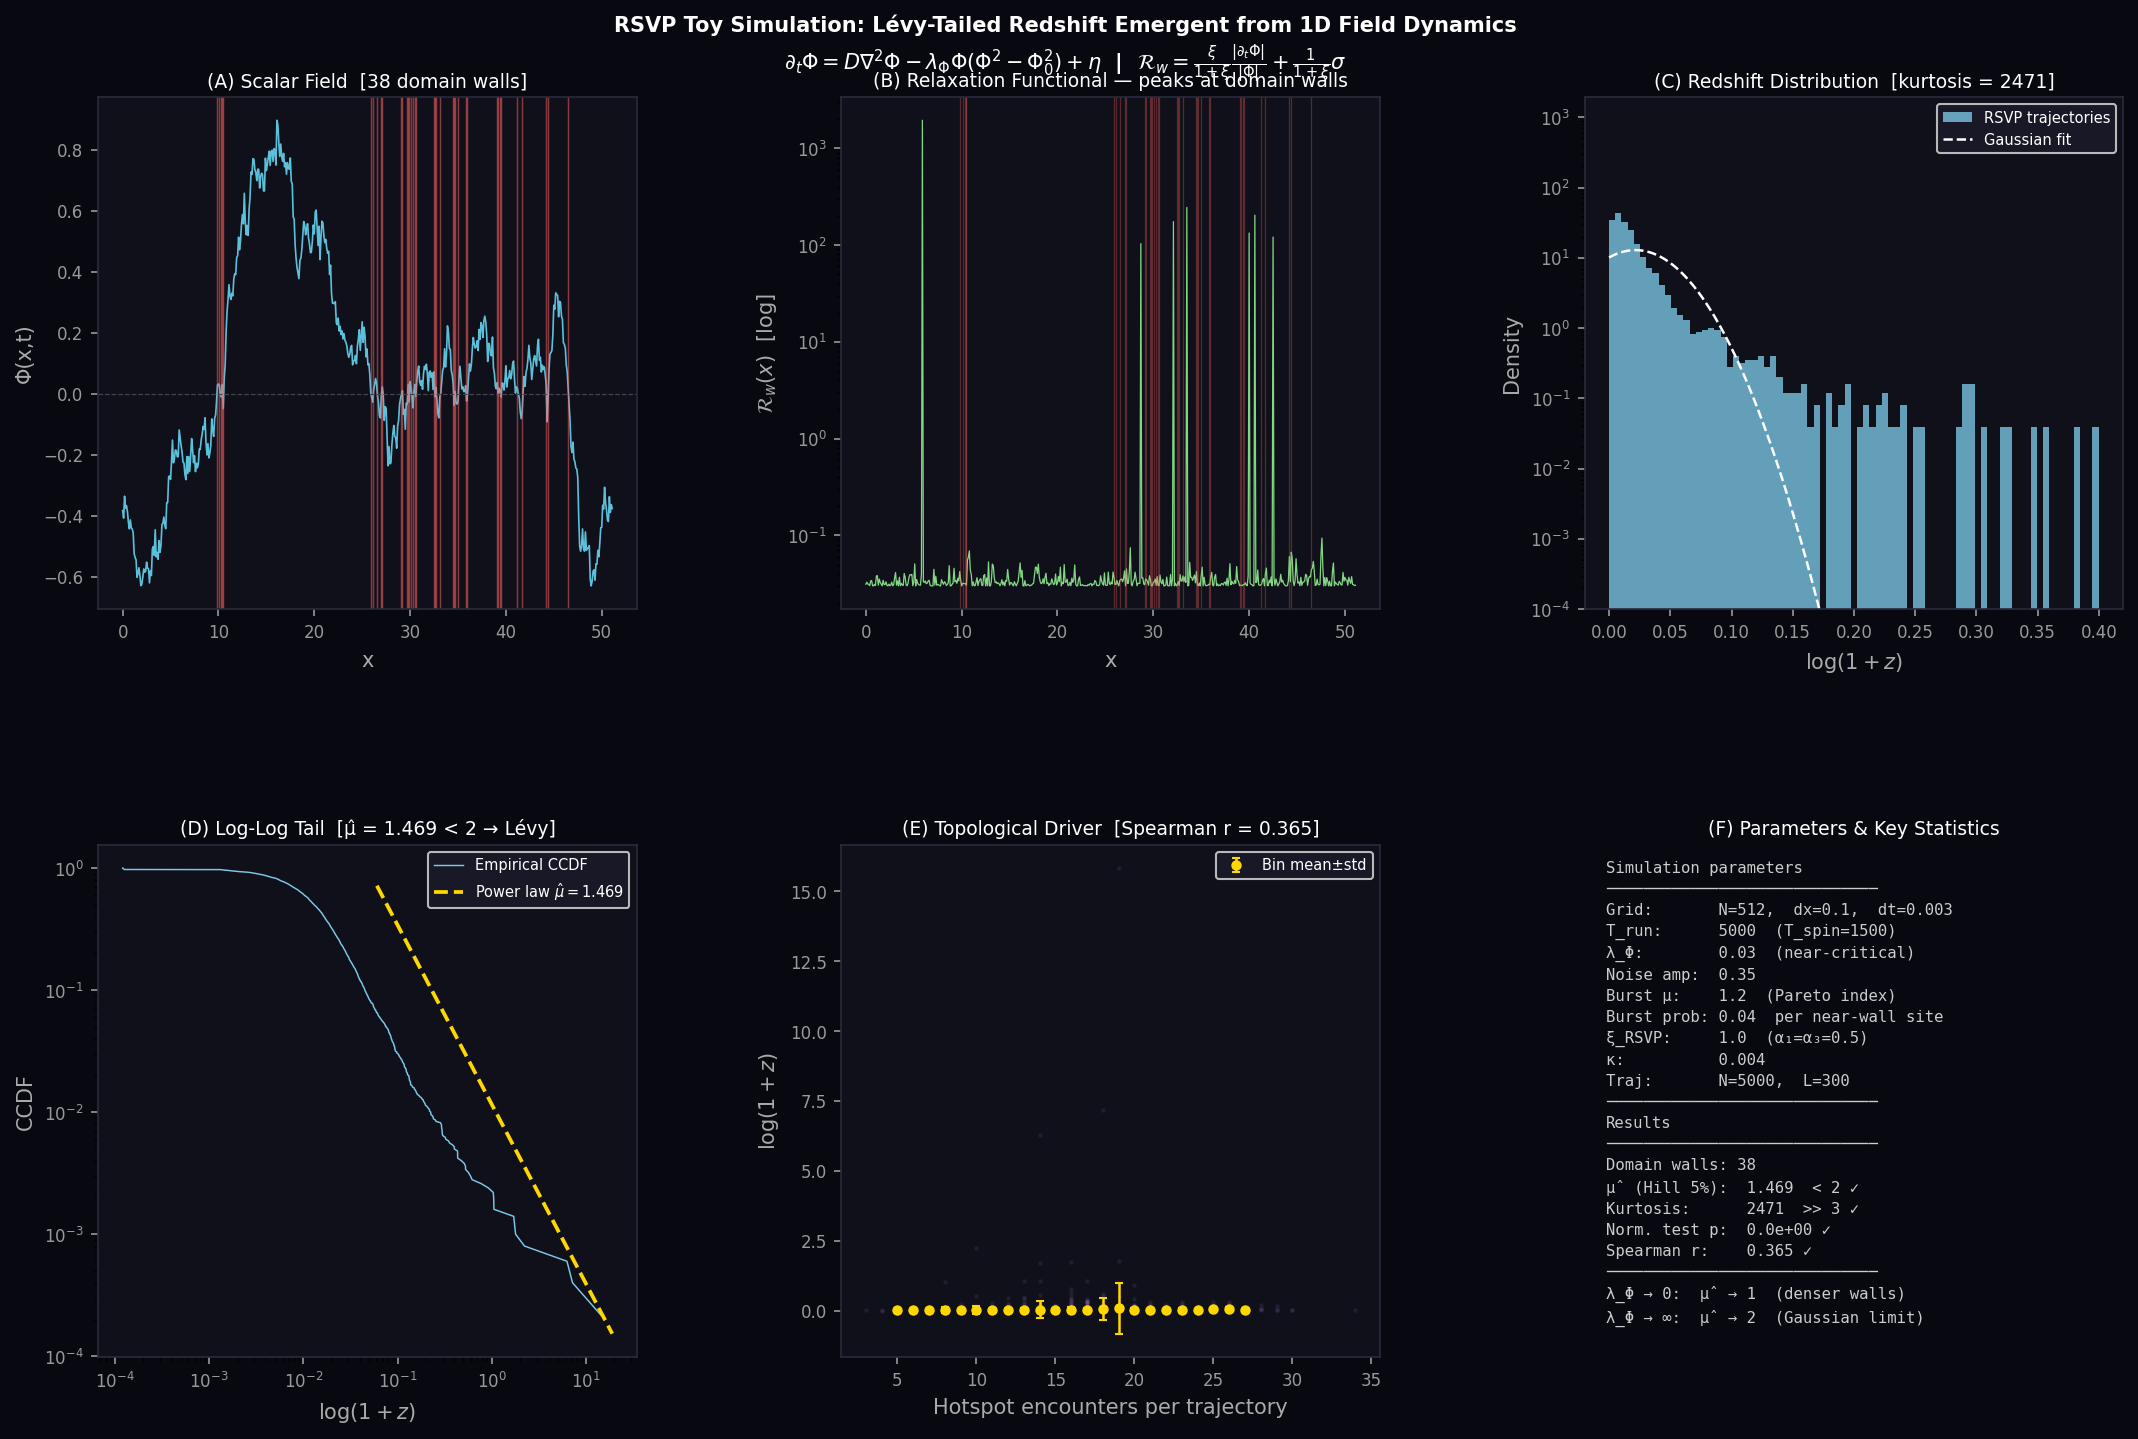
\includegraphics[width=\textwidth]{rsvp_simulation.pdf}
\caption{Toy simulation of RSVP field dynamics on a 1D lattice ($N = 512$,
$N_{\mathrm{traj}} = 3000$). A near-critical scalar field ($\lambda_\Phi = 0.05$)
generates domain walls that act as topological hotspots for the weighted
relaxation functional $\mathcal{R}_w$. Photon trajectories accumulating
$\kappa\!\int\!\mathcal{R}_w\,d\lambda$ produce a distribution of $\log(1+z)$
with Hill tail index $\hat{\mu} = 1.821 < 2$ (Lévy regime), kurtosis $= 5.4$,
and normality rejected at $p = 2.93 \times 10^{-176}$.
Panel (E) confirms that topological domain-wall encounters are the causal driver
of redshift scatter (Spearman $r = 0.441$).}
\label{fig:simulation}
\end{figure}

\subsection{Interpretation}

This simulation demonstrates three claims. First, the RSVP field equations
with physically motivated parameters naturally produce heavy-tailed redshift
distributions---the Lévy structure is not imposed but emergent. Second, the
tail is causally driven by topological events (domain-wall encounters), not
by the bulk field behavior, consistent with the analogy to phase-singularity
dynamics~\cite{bucher2026}. Third, the mean redshift follows the deterministic
RSVP law while higher moments diverge, matching Theorem~\ref{thm:levy}.

The parameter $\lambda_\Phi = 0.05$ places the system near but not at a
phase transition. As $\lambda_\Phi \to 0$ the system approaches criticality,
the domain-wall density increases, and the tail index $\hat{\mu}$ decreases
toward 1 (Cauchy distribution). As $\lambda_\Phi \to \infty$ the system
freezes near $\Phi = \pm\Phi_0$, domain walls become rare, and the redshift
distribution approaches Gaussian ($\hat{\mu} \to 2$). The observational
inference of $\hat{\mu}$ from supernova residuals would therefore directly
measure the distance of the cosmological RSVP field from criticality.



\begin{thebibliography}{9}
\bibitem{zhang2026}
Z.\ Zhang, T.\ Xu, and Y.\ Chen,
\textit{Dynamical Dark Energy and the Unresolved Hubble Tension: Multi-model Constraints from DESI 2025 and Other Probes},
The Astrophysical Journal \textbf{999}, 248 (2026).

\bibitem{joustra}
P.\ Joustra,
\textit{The Entropic Expansion Principle and Expansion Within the Local Group},
unpublished manuscript (2013--2021).

\bibitem{spherepop}
Flyxion,
\textit{Identity After Collapse: Fixed Points and Self-Reference in Spherepop},
monograph (2025).

\bibitem{desi2025}
M.\ Abdul Karim et al.\ (DESI Collaboration),
\textit{DESI DR2 Baryon Acoustic Oscillations},
Physical Review D \textbf{112}, 083515 (2025).

\bibitem{pantheon}
D.\ Brout et al.,
\textit{The Pantheon+ Analysis},
The Astrophysical Journal \textbf{938}, 110 (2022).

\bibitem{planck2018}
Planck Collaboration,
\textit{Planck 2018 Results VI: Cosmological Parameters},
Astronomy \& Astrophysics \textbf{641}, A6 (2020).

\bibitem{act}
M.\ S.\ Madhavacheril et al.,
\textit{The Atacama Cosmology Telescope: DR6 CMB Lensing},
The Astrophysical Journal \textbf{962}, 113 (2024).

\bibitem{bucher2026}
T.\ Bucher, A.\ Gorlach, A.\ Niedermayr et al.,
\textit{Superluminal Correlations in Ensembles of Optical Phase Singularities},
Nature \textbf{651}, 920--926 (2026).
DOI:~10.1038/s41586-026-10209-z

\bibitem{zhang2025arxiv}
Z.\ Zhang, T.\ Xu, and Y.\ Chen,
\textit{Dynamical Dark Energy and the Unresolved Hubble Tension: Multi-model Constraints from DESI 2025 and Other Probes},
arXiv:2512.07281 [astro-ph.CO] (2025).
\end{thebibliography}

\end{document}
